\documentclass[class=article]{standalone}

%\documentclass[12pt]{article}
%
%\usepackage{../preambolo}

\begin{document}
	\section{Il Sistema}
	Nel capitolo seguente verrà trattato il sensore che è stato montato sulla bicicletta al fine di raccogliere i dati necessari per lo svolgimento di questa tesi. 
%	Verrà inoltre fornita una panoramica su cosa ci aspettiamo di vedere dai dati raccolti dallo stesso durante le prove effettuate.
	
	\begin{figure}[h]
		\begin{subfigure}[h]{0.5\textwidth}
			\centering\includegraphics[width=0.9\linewidth]{./img/bicicletta2.jpg}
			\caption{}
			\label{fig:bici}
		\end{subfigure}
		\begin{subfigure}[h]{0.5\textwidth}
			\centering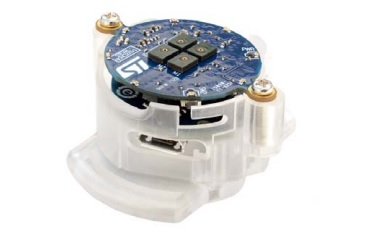
\includegraphics[width=0.8\linewidth]{./img/bluecoin.jpg}
			\caption{}
			\label{fig:sensore}
		\end{subfigure}
		
		\caption[]{La bicicletta \ref{fig:bici} e il sensore \ref{fig:sensore} usati durante le uscite per acquisire i dati}
	\end{figure}
	
	\subsection{Il Sensore}
	Il sensore utilizzato per raccogliere i dati è il Blue Coin della ST Microelettronics (\url{https://www.st.com/en/evaluation-tools/steval-bcnkt01v1.html}) sulla quale è stato montato il software \(FP\_ALLMEMS1\_V4.3.0\) presente sulla pagina web del produttore.\hfill\break
	
	Questo sensore è dotato di
	\begin{itemize}
		\item Accelerometro: misura in \(mg\) (millesimi dell'accelerazione gravitazionale) l'accelerazione lungo gli assi x,y e z. Successivamente convertita in \(m/s^2\)
		\item Giroscopio: misura in \(mdps\) la velocità angolare attorno agli angoli di rollio (\(roll\)), beccheggio (\(pitch\)) e imbardata (\(yaw\)). Convertita, in seguito, in \(dps\)
		\item Magnetometro: misura in \(mG\) (\(milli Gauss\)) l'intensità del campo magnetico, può essere utilizzato per determinare l'orientamento. Convertita in \(\mu T\)
		\item Barometro: misura la pressione atmosferica in \(mBar\)
		\item Termometro: misura la temperatura in gradi \(^{\circ}C\)
		\item Microfono
	\end{itemize}
	
	Durante i nostri esperimenti sono stati utilizzati solo i dati provenienti dall'accelerometro, dal giroscopio e dal magnetometro in quanto sufficienti per ottenere i risultati da noi cercati.
		
	Il sensore è stato montato di volta in volta sul telaio della bicicletta, sull'asse che dalla sella prosegue verso il manubrio, al di sotto di quest'ultimo. Sfortunatamente, in questo modello di bicicletta, quest'asse è inclinato rispetto all'orizzontale e leggermente curvo. Questo ha reso necessario trovare un modo per calcolare la rotazione dei dati al fine di far coincidere gli assi del sensore e con quelli della bicicletta, ma di questo tratteremo nel prossimo capitolo.\hfill\break
	
	\begin{center}
		\begin{figure}[h!]
			\begin{subfigure}[h]{.5\textwidth}
				\centering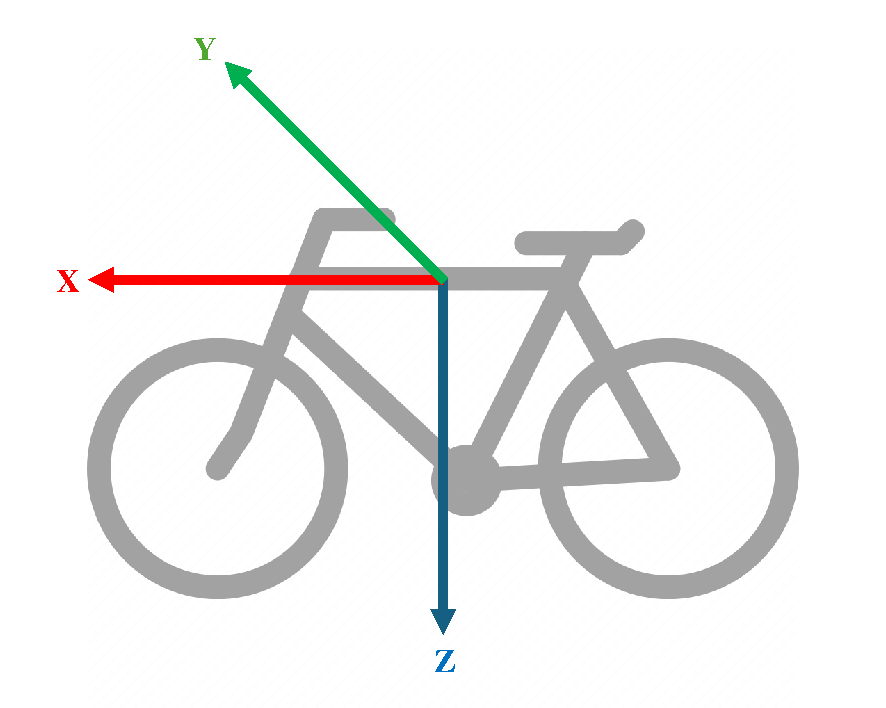
\includegraphics[width=.9\textwidth]{img/axis}
				\caption[]{Bicicletta con il sistema di riferimento usato}
				\label{fig:axes}
			\end{subfigure}
			\begin{subfigure}[h]{.5\textwidth}
				\centering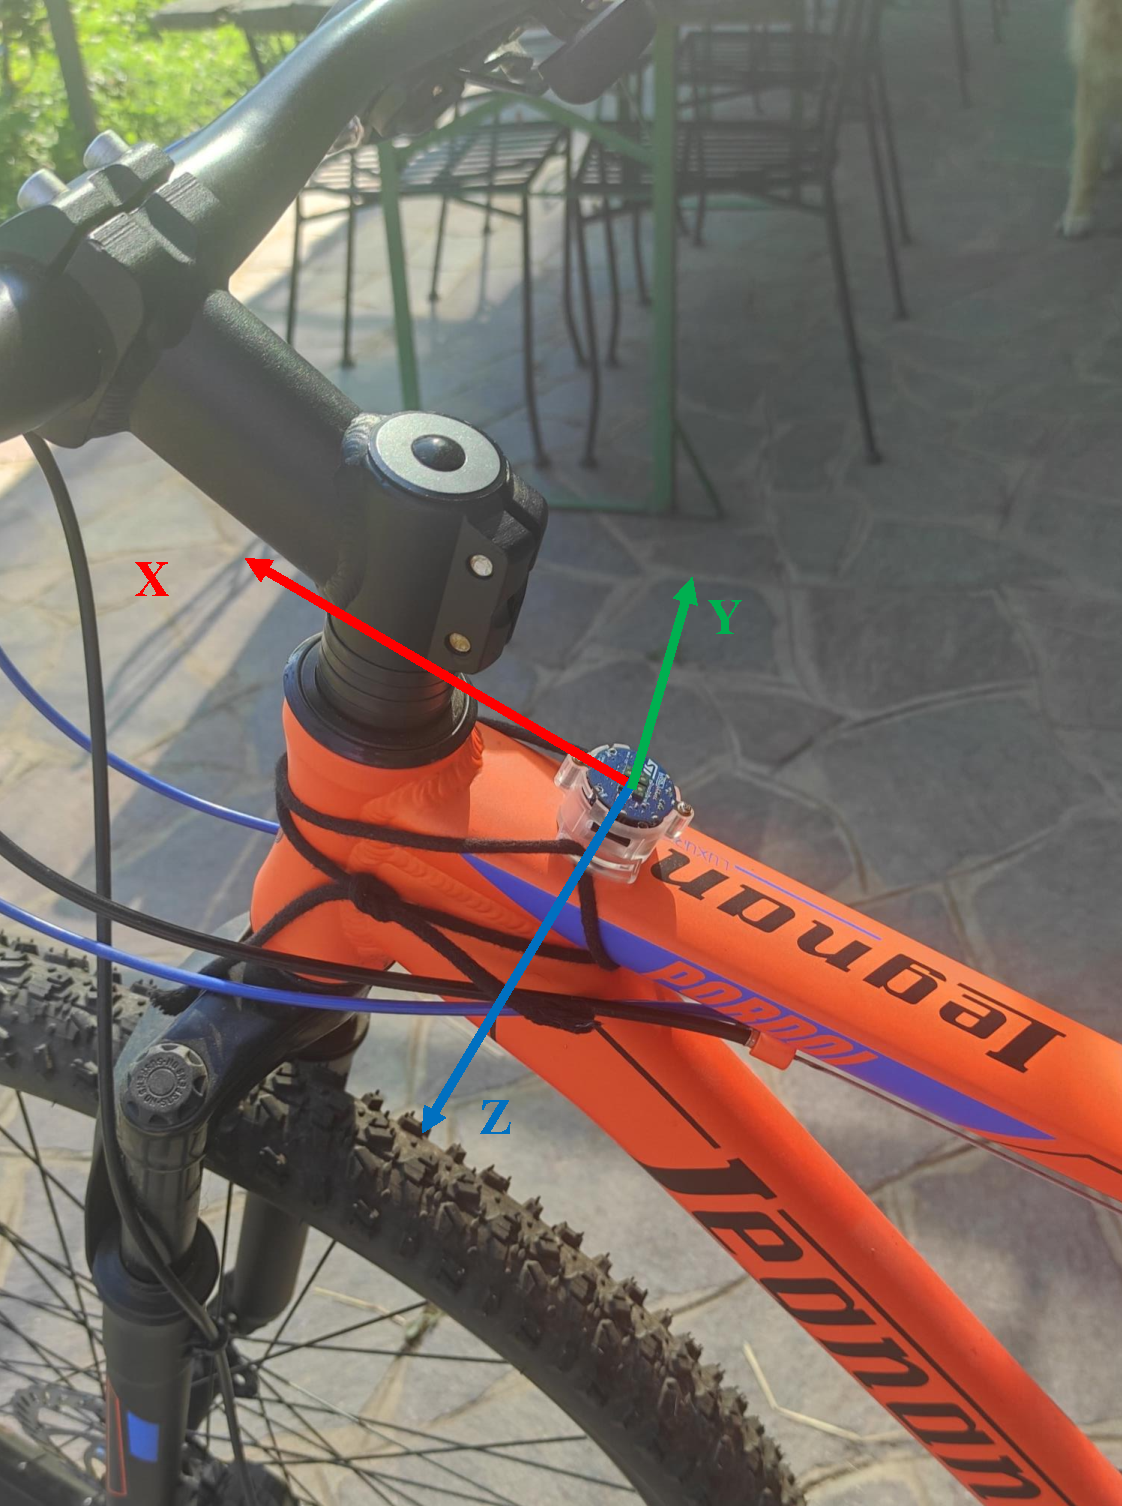
\includegraphics[width=.7\textwidth]{img/SensorAxes}
				\caption[]{Il sensore, con il suo sistema di riferimento, montato sulla bicicletta}
				\label{fig:SensorAxes}
			\end{subfigure}
		\end{figure}
	\end{center}
	
	Il sistema di riferimento usato dal sensore è quello \(NED\) (north-east-down), avremo quindi che: la direzione positiva dell'asse \(x\) sarà quella di movimento della bicicletta (di fronte a noi), l'asse \(y\) avrà direzione positiva sul lato destro della bicicletta e l'asse \(z\) sarà diretto verso il basso.
	Da notare che, nonostante sia diretta verso il basso, il sensore percepisce l'accelerazione gravitazionale come negativa in quanto, non vedendo i risultati della stessa (il sensore non sta precipitando), "ritiene" che ci sia un'accelerazione negativa (rivolta verso l'alto) che gli sta impedendo di cadere. 
	In altre parole, il sensore rileva la reazione vincolare della superficie terrestre, che è una forza normale che contrasta la gravità e mantiene il sensore in equilibrio.
	
	
%	\subsection{I Dati Raccolti}
%	In questa sezione andremo a trattare i dati rilevati dal sensore durante 
%	\subsubsection{Accelerazioni}
%	\subsubsection{Velocità Angolari}
%	\subsubsection{Campo Magnetico}
	
\end{document}